\documentclass[11pt]{article}

\usepackage[margin=1in]{geometry}
\usepackage{amsmath,amssymb}
\usepackage{booktabs}
\usepackage{array}
\usepackage{enumitem}
\usepackage{hyperref}
\usepackage{xcolor}
\usepackage{pgfplots}
\pgfplotsset{compat=1.18}
\usepgfplotslibrary{groupplots}
\usepackage{caption}

\hypersetup{colorlinks=true, linkcolor=blue!50!black, citecolor=green!40!black,
            urlcolor=blue!60!black}

\newcommand{\pcorrect}{P(\text{correct})}

\title{\textbf{A Belief-Engine Decision Model for Normalizing\\
Scraped E-Commerce Product Specifications}\\[4pt]
\large From belief and cost to \emph{information}: which clue to buy next, and when
to stop --- a thinking-first prototype that decides, per field, whether a value is
safe to publish}

\author{Chirag \\ \small AI-Native Engineering deliverable (Cohort 3), Weeks 1--2 combined}
\date{\today}

\begin{document}
\maketitle

\begin{abstract}
\noindent
Scraping product data is the easy part; deciding whether a scraped value is
\emph{correct} is the hard part, because the true canonical specification is never
observed at decision time. We model each scraped field (e.g.\ \texttt{ram\_gb},
\texttt{storage\_gb}, \texttt{weight\_g}) as one of six mutually-exclusive hidden
``worlds'' (\textsf{correct}, \textsf{unit\_error}, \textsf{wrong\_product},
\textsf{typo}, \textsf{missing}, \textsf{garbled}), start from a source-reliability
prior, update it with cheap evidence signals via Bayes' rule, and choose among
\textsc{accept}, \textsc{repair}, \textsc{buy-more-evidence},
\textsc{flag-for-human}, and \textsc{reject} by \emph{minimum expected loss} under an
asymmetric cost matrix in which publishing a wrong value is by far the most
expensive outcome. We evaluate on 40 labelled cases (labels hidden at decision time)
against an autonomous no-human variant and a deliberately ``dumb'' score-plus-threshold
baseline. On this small sample the full policy attains the lowest average decision
cost (2.30 vs.\ 3.10 for the baseline; paired Wilcoxon $p\approx0.015$), but with
three important honesty caveats: (i) the win is \emph{narrow}---the median per-case
cost difference is $0$ and only 9 of 40 cases differ; (ii) all three policies commit
the same two catastrophic wrong-publishes, so the belief layer buys its lower average
cost mostly by escalating 57.5\% of cases to a human rather than by preventing the
expensive errors; and (iii) the model's top confidence bin is empirically only
$\sim$60\% correct, which---if real---would invert the very
\textsc{accept} decision the expected-loss rule is meant to make. We therefore
present this as a \emph{calibrated way of thinking} about the problem, not a
production system, and we are explicit about which numbers are assumptions and which
are measured. We then add an \emph{information layer}: we measure the agent's doubt in
\emph{bits} (Shannon entropy), rank candidate evidence by \emph{expected information
gain per unit cost}, and replace the earlier flat two-buy cap with a true
\emph{value-of-information} (VOI) stop rule. Three findings stand out and are honest
about their own limits: (a) a clue can flip which world leads while barely reducing
entropy (the leading out-of-support signal cuts doubt by only $0.24$ of $2.12$ bits);
(b) the most \emph{informative} clue is not the best \emph{buy} once cost enters (the
manufacturer proxy leads on raw bits but a cheaper cross-source panel wins on
bits-per-cost); and (c) under our own cost matrix \emph{every} candidate clue has
\emph{zero} value of information---the guaranteed human-review cost (\textsc{flag}$=2$)
is such a strong ceiling that the agent should flag, not buy, and we show by
prediction-and-test that even making the human much more expensive does \emph{not}
rescue buying on this high-entropy case (VOI plateaus below the clue cost), because no
single clue can concentrate belief enough to escape into a cheaper action. All priors, likelihoods, and costs are author-stated assumptions with recorded
provenance; three adversarial AI reviews and five human discussions shaped the design
and are documented alongside.
\end{abstract}

\tableofcontents

\section{Introduction and problem statement}
\label{sec:intro}

E-commerce catalogs are assembled from scraped and syndicated data: the same phone's
specifications are pulled from manufacturer pages, retailer listings, and price
aggregators, then normalized into one record. Scraping itself is largely solved; the
expensive, unglamorous problem is deciding whether a scraped \emph{value} is
trustworthy enough to publish. A field can be perfectly parseable and still wrong:
\texttt{16000\,MB} of RAM (a unit slip), \texttt{160\,GB} of RAM (an impossible
typo), \texttt{512\,GB} of storage that is real but belongs to a different variant,
or a numeric value that five sites agree on only because they all copied the same bad
upstream feed.

The defining difficulty is that \textbf{the true canonical specification is never
observed at decision time}. The agent sees clues---the value, its plausibility, what
other sources say---but never the ground truth. This is a decision-under-uncertainty
problem, not a classification problem, and the right tool is a \emph{belief} over what
might have happened, combined with a \emph{cost} of being wrong.

\paragraph{The decision.} For each scraped field the agent must choose one of:
\begin{itemize}[nosep]
  \item \textsc{accept} --- publish the value as-is;
  \item \textsc{repair} --- transform then publish (e.g.\ \texttt{16000\,MB}
        $\rightarrow$ \texttt{16\,GB});
  \item \textsc{buy} --- pay to gather more evidence (re-scrape, query a manufacturer
        proxy) before deciding;
  \item \textsc{flag} --- send to a human reviewer;
  \item \textsc{reject} --- drop the value (publish nothing for this field).
\end{itemize}

\paragraph{Scope.} We work in consumer electronics (phones/laptops), one decision per
scraped field. We assume the upstream step correctly identified \emph{which} field a
value belongs to; schema/key-mismatch across sources is out of scope and revisited as
a limitation (\S\ref{sec:limitations}).

\paragraph{Contributions and honest framing.} This is a thinking-first prototype
combining two deliverables. Its contribution is a \emph{calibrated way of thinking}:
an explicit, auditable pipeline from source-reliability prior, through Bayesian
updates on cheap signals, to a minimum-expected-loss decision with a human escape
hatch, \emph{extended with an information layer} that measures doubt in bits, ranks
evidence by expected information gain per unit cost, and decides when to stop buying
by true value of information (\S\ref{sec:info}). Every prior, likelihood, and cost is
an author-stated assumption with recorded provenance (\S\ref{sec:assumptions}); we
never present a guess as a measured fact. The empirical results (\S\ref{sec:results})
are deliberately reported with their caveats: a small sample, a cost advantage that is
statistically real but \emph{narrow}, and a calibration problem in the highest-stakes
confidence bin. The information analysis adds its own honest twist---under our cost
matrix, most doubtful cases have zero value of information, so the agent should flag
rather than buy, revealing that the buy policy was silently driven by an optimistic
flat human-review cost.

\section{Related work and positioning}
\label{sec:related}

The components here are standard; the contribution is their explicit, honest
assembly for a concrete data-quality task.

\begin{itemize}[nosep]
  \item \textbf{Bayesian decision theory.} Choosing the action with minimum expected
        loss under a posterior is the textbook Bayes decision rule~\cite{berger1985},
        and the prior$\rightarrow$likelihood$\rightarrow$posterior update with
        weakly-informative priors follows standard practice~\cite{gelman2013bda}.
  \item \textbf{Reject-option classification.} Our ``act only above a cost-derived
        confidence, otherwise abstain to a human'' rule is exactly Chow's reject
        option~\cite{chow1970}: the \textsc{flag} action is a principled abstain, not
        an admission of defeat.
  \item \textbf{Cost-sensitive learning.} The asymmetric cost matrix and the insight
        that one must not simply pick the most-likely class under asymmetric losses
        is Elkan's cost-sensitive framing~\cite{elkan2001}.
  \item \textbf{Calibration.} That predicted probabilities must match empirical
        frequencies---and that modern models are often overconfident---motivates our
        calibration analysis and the recalibration remedies (Platt/temperature/isotonic
        scaling)~\cite{guo2017calibration,platt1999,zadrozny2002}.
  \item \textbf{Sequential testing / value of information.} The ``buy evidence then
        re-decide'' loop is, in its fully-correct form, a sequential decision
        problem~\cite{wald1945sprt}; we use a budget heuristic and say so
        (\S\ref{sec:policy}).
  \item \textbf{Active learning and product matching.} Our human-in-the-loop routing
        is an active-learning setup~\cite{settles2009active}, which biases evaluation
        (\S\ref{sec:threats}); the \textsf{wrong\_product} problem connects to
        large-scale product matching benchmarks such as WDC
        Products~\cite{primpeli2019wdc}.
\end{itemize}

\noindent
Where an idea came from an online discussion or the course rather than a paper, we say
so in-text rather than manufacture a citation.

\section{Hidden states: six MECE worlds}
\label{sec:worlds}

The hidden reality behind a value is exactly one of six worlds, chosen to be
mutually exclusive and collectively exhaustive (MECE). A tie-breaker, applied in
order, guarantees a value never sits in two boxes: (1) unparseable as this field
$\rightarrow$ \textsf{garbled}; (2) empty/placeholder $\rightarrow$ \textsf{missing};
(3) parses to a number $\rightarrow$ decide among the remaining worlds using the
plausibility (``support'') and unit-conversion tests.

\begin{center}
\begin{tabular}{@{}l p{0.72\linewidth}@{}}
\toprule
\textbf{World} & \textbf{The reality that produced the value} \\
\midrule
\textsf{correct} & Value matches the true canonical spec for this product+field. \\
\textsf{unit\_error} & Right magnitude, wrong unit (\texttt{16000\,MB}$\to$\texttt{16\,GB}). Narrow by design; a broader class of \emph{measurement-definition} errors (net vs.\ gross weight, diagonal vs.\ width) is noted as future work. \\
\textsf{wrong\_product} & A valid, in-support value taken from a different product/variant/revision (includes \emph{stale}). Looks normal in isolation. \\
\textsf{typo} & Transcription slip producing an off/out-of-support number (\texttt{160\,GB} RAM). \\
\textsf{missing} & Empty/null/placeholder-empty. \\
\textsf{garbled} & Present but unparseable as this field (encoding junk, HTML, ``N/A''). \\
\bottomrule
\end{tabular}
\end{center}

\noindent
When the agent cannot tell two worlds apart from the value alone, that is
\emph{belief uncertainty}: it splits probability mass across the live worlds; it does
not merge the boxes. Distinguishing \textsf{typo} from \textsf{wrong\_product} is
justified by \emph{decision relevance}---they lead to different repairs (fix the digit
vs.\ re-identify the product), so they must be separate states.

\section{The belief model}
\label{sec:belief}

\subsection{Source-reliability prior}
Before seeing evidence, the agent starts from a prior over the six worlds that depends
only on \emph{where the value came from}. We use three source tiers---manufacturer
(\textsc{mfr}), mid-reliability retail (\textsc{mid}), and sketchy aggregator
(\textsc{sky})---each expressed as 100 tokens split over the worlds. The
mid-reliability board is the anchor:
\[
\begin{aligned}
\text{\textsc{mid}: }\ &\pcorrect=0.50,\ \textsf{unit\_error}=0.10,\ \textsf{wrong\_product}=0.15,\\
&\textsf{typo}=0.05,\ \textsf{missing}=0.10,\ \textsf{garbled}=0.10.
\end{aligned}
\]
\textsc{mfr} shifts mass toward \textsf{correct} ($0.80$); \textsc{sky} away from it
($0.30$). These are \emph{weakly-informative} priors: strong enough to rule out the
absurd (via support ranges, a phone cannot have ``100\,ft of RAM'') but not so strong
they override real evidence.

\subsection{Likelihoods}
The likelihood answers the backwards question: \emph{if this world were true, how
naturally would it produce this evidence signal?} Each $P(\text{signal}\mid
\text{world})$ lives in $[0,1]$ and the values \emph{do not} sum to one across
worlds---they are per-world sampling probabilities, not a distribution over worlds.
The primary signal is ``out-of-support'' (\textsf{oos}); for a value like
\texttt{160\,GB} RAM the likelihoods are $P(\textsf{oos}\mid\textsf{typo})=0.90$,
$P(\textsf{oos}\mid\textsf{unit\_error})=0.40$,
$P(\textsf{oos}\mid\textsf{wrong\_product})=0.10$,
$P(\textsf{oos}\mid\textsf{correct})=0.02$, and $0.01$ for
\textsf{missing}/\textsf{garbled} (a parsed number is essentially never empty or junk).

\emph{Rigor note.} For a binary support test the ``in-support'' case implicitly uses
$1-P(\textsf{oos}\mid\text{world})$. For any multi-valued signal (e.g.\ cross-source
$\in\{\text{agree},\text{disagree},\text{absent}\}$) the conditional distribution must
sum to one \emph{over the evidence outcomes} for a fixed world, or the ``absent''
outcome silently leaks probability mass.

\subsection{Bayesian update and chaining}
The posterior is prior$\times$likelihood, renormalized:
\begin{equation}
P(\text{world}\mid e) \;=\; \frac{P(\text{world})\,P(e\mid\text{world})}
{\sum_{w} P(w)\,P(e\mid w)}.
\label{eq:bayes}
\end{equation}
On the \texttt{160\,GB}-RAM \textsc{mid} example, the single \textsf{oos} signal moves
the board to $\textsf{typo}=0.402$, $\textsf{unit\_error}=0.357$,
$\textsf{wrong\_product}=0.134$, $\pcorrect=0.089$, and $0.009$ each for the empty
worlds. Note the base-rate discipline: \textsf{typo} lands at $0.40$, not $0.95$,
precisely because its prior was low---striking evidence does not erase the prior.

Multiple clues chain: the posterior of one update becomes the prior of the next
(Eq.~\ref{eq:bayes} applied repeatedly). \textbf{This asserts conditional independence
of the signals given the world,}
$P(e_1,e_2\mid w)=P(e_1\mid w)\,P(e_2\mid w)$, an assumption we state openly because it
is questionable for our signals: a typo that pushes a value out of support will
\emph{also} tend to make it disagree with other sources---one latent cause, two
signals---so chaining them double-counts and over-concentrates the posterior. This is
the likely mechanistic root cause of the over-confidence we measure in
\S\ref{sec:results}. Principled fixes (a joint likelihood for correlated signal groups,
or a naive-Bayes-style weight-of-evidence discount) are future work.

\section{Assumptions, provenance, and the cost matrix}
\label{sec:assumptions}

\subsection{What is assumed vs.\ measured}
The priors, likelihoods, and costs are \textbf{author-stated assumptions}, informed by
experience browsing major B2C retail sites---not counts from a labelled dataset. We
label them as such on purpose: a number without its provenance is ``a guess wearing a
lab coat.'' The only \emph{measured} quantities in this paper are the evaluation
results of \S\ref{sec:results}, computed by running the model over labelled cases.
Because the derived thresholds and posteriors are computed \emph{from} the assumptions,
they inherit the assumptions' uncertainty: every ``derived floor'' or posterior below
should be read as ``given these stated assumptions.''

\subsection{Asymmetric cost matrix}
Not all mistakes cost the same; publishing a wrong value dominates. Costs are relative
pain units, author-assigned on the principle ``whatever ends up publishing wrong data
is most expensive.'' Table~\ref{tab:cost} gives cost(action, true world).

\begin{table}[h]
\centering
\caption{Asymmetric cost matrix (author-stated assumption). Rows are actions, columns
are the true world; lower is better. \textsc{accept} on any flaw is the worst outcome.}
\label{tab:cost}
\begin{tabular}{@{}l cccccc@{}}
\toprule
Action $\downarrow$ / World $\rightarrow$ & \textsf{correct} & \textsf{unit\_err} & \textsf{wrong\_prod} & \textsf{typo} & \textsf{missing} & \textsf{garbled} \\
\midrule
\textsc{accept} & 0 & 20 & 20 & 20 & 20 & 20 \\
\textsc{repair} & 18 & 0 & 8 & 4 & 12 & 12 \\
\textsc{buy}    & 1 & 1 & 1 & 1 & 1 & 1 \\
\textsc{flag}   & 2 & 2 & 2 & 2 & 2 & 2 \\
\textsc{reject} & 5 & 6 & 6 & 2 & 1 & 1 \\
\bottomrule
\end{tabular}
\end{table}

\noindent
The asymmetry ($20$ for a wrong publish vs.\ $1$--$2$ for buying/flagging) is what
makes the problem interesting: even when \textsf{correct} is the single most likely
world, a modest chance of a costly flaw can make \textsc{accept} the higher-cost choice.

\section{Policy: minimum expected loss with an abstain option}
\label{sec:policy}

\subsection{Decision rule}
For each action $a$, its expected loss under the current belief is
\begin{equation}
\mathbb{E}[\text{loss}\mid a] \;=\; \sum_{\text{world}} P(\text{world})\,\text{cost}(a,\text{world}),
\label{eq:eloss}
\end{equation}
and the agent takes the action with the smallest expected loss. On the
\texttt{160\,GB} posterior above, this yields $\mathbb{E}[\textsc{accept}]\approx18.2$,
$\mathbb{E}[\textsc{repair}]\approx4.5$, $\mathbb{E}[\textsc{reject}]\approx4.0$,
$\mathbb{E}[\textsc{flag}]=2.0$, and $\mathbb{E}[\textsc{buy}]=1.0$: the engine's
answer is \emph{don't guess---buy more evidence}, a non-obvious decision produced by
the model rather than by hand.

\subsection{Derived \textsc{accept} threshold (Chow's reject option)}
\textsc{accept} (cost 20 if wrong, 0 if right) beats \textsc{flag} (flat 2) only when
$(1-\pcorrect)\times 20 < 2$, i.e.\ $\pcorrect > 0.90$. So $90\%$ is the
cost-\emph{derived} floor; we operate at a more conservative $95\%$ for a publishing
safety margin. Acting only above a cost-derived confidence and otherwise abstaining to
a human is precisely Chow's reject-option rule~\cite{chow1970}.

\subsection{Buying information: a budget heuristic, not true VOI}
Whether to \textsc{buy} is governed by two rules. (i) A \emph{value-of-information
pre-filter}: if buying cannot change the action (e.g.\ \textsf{missing}/\textsf{garbled}
dominate, or every plausible world already implies the same action), do not buy.
(ii) A \emph{cost cap}: since \textsc{flag} costs 2 and guarantees a resolution, never
spend more than 2 on buying---a hard cap of two \textsc{buy}s, then \textsc{flag}.
We are explicit that this is a \textbf{budget heuristic, not true value of
information}: true VOI compares $\mathbb{E}[\text{loss now}]$ against
$\mathbb{E}[\text{loss after the evidence}]$ and buys only if the expected reduction
exceeds the fetch cost. The heuristic needs only a counter, no forecasting; its
fully-correct form is a sequential/optimal-stopping problem~\cite{wald1945sprt}, out
of scope here. Section~\ref{sec:info} replaces this heuristic with a true VOI rule and
shows it makes a materially different decision on the worked case.

\section{The information layer: bits, which clue to buy, and when to stop}
\label{sec:info}

The policy above answers \emph{what to do given a belief}; it never asks \emph{how
much doubt remains} or \emph{which evidence is worth buying}. This section adds that
information layer on the same worked case (\textsf{ram\_gb}$=160$), reusing the
posterior of \S\ref{sec:belief} and the cost matrix of \S\ref{sec:assumptions}. No new
assumptions are introduced beyond the per-clue likelihoods stated in
Table~\ref{tab:clues}; all numbers are reproduced by a standard-library script.

\subsection{Measuring doubt in bits}
We quantify total uncertainty with Shannon entropy $H(b)=-\sum_w b(w)\log_2 b(w)$,
in bits. For six equally likely worlds $H=\log_2 6=2.585$ bits (the ceiling). The
``mid''-reliability prior sits at $H=2.123$ bits---already very unsure. After the
single \emph{out-of-support} clue the posterior
\[
b_{\text{post}}=(0.089,\,0.134,\,0.357,\,0.402,\,0.009,\,0.009)
\]
has $H=1.880$ bits, an \emph{observed} information gain of only $0.243$ bits.

\begin{center}
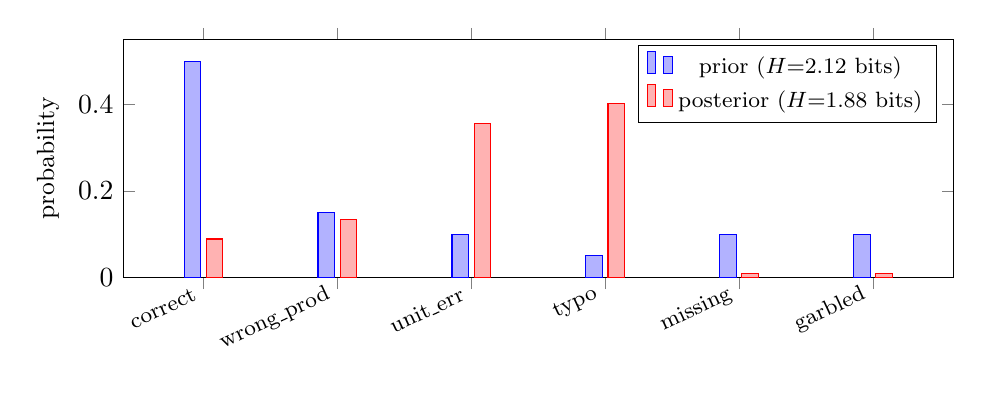
\begin{tikzpicture}
\begin{axis}[
  width=\linewidth, height=4.6cm, ybar, bar width=6pt,
  ymin=0, ymax=0.55, ylabel={probability}, ylabel style={font=\small},
  symbolic x coords={correct,wrong\_prod,unit\_err,typo,missing,garbled},
  xtick=data, x tick label style={rotate=25,anchor=east,font=\footnotesize},
  legend style={font=\footnotesize,at={(0.98,0.98)},anchor=north east},
  enlarge x limits=0.12]
\addplot coordinates {(correct,0.50)(wrong\_prod,0.15)(unit\_err,0.10)(typo,0.05)(missing,0.10)(garbled,0.10)};
\addplot coordinates {(correct,0.089)(wrong\_prod,0.134)(unit\_err,0.357)(typo,0.402)(missing,0.009)(garbled,0.009)};
\legend{prior ($H{=}2.12$ bits), posterior ($H{=}1.88$ bits)}
\end{axis}
\end{tikzpicture}
\captionof{figure}{The out-of-support clue \emph{flips the leader}
(\textsf{correct}$\to$\textsf{typo}) yet barely reduces entropy ($-0.24$ bits):
changing the top-ranked world is not the same as reducing doubt.}
\label{fig:entropy}
\end{center}

\subsection{Expected vs.\ observed gain}
The $0.243$ bits above is the gain \emph{after} seeing \textsf{oos}$=$true. Before
running the check the outcome is unknown: \textsf{oos}$=$true occurs with probability
$P(\textsf{oos})=\sum_w b(w)P(\textsf{oos}\mid w)=0.112$ (then $H=1.880$), and
\textsf{oos}$=$false with probability $0.888$ (then $H=1.897$). The honest value of
\emph{running} the check is the conditional entropy
$H(W\mid \text{clue})=0.112(1.880)+0.888(1.897)=1.895$ bits, giving an
\textbf{expected information gain} of $2.123-1.895=0.228$ bits. Expected gain equals
the mutual information between clue and hidden world; ranking clues by the
\emph{observed} number instead is a standard error, and we avoid it below.

\subsection{Which clue to buy next: expected bits per unit cost}
Three costed clues are available (a manufacturer spec-page proxy, a reference-dataset
SKU lookup, and cross-source agreement). Table~\ref{tab:clues} states their
two-outcome likelihoods (author assumptions) and the resulting expected gain and
bits-per-cost, computed from the post-oos posterior.

\begin{table}[h]\centering\small
\caption{Ranking candidate clues on the worked case. The \emph{most informative} clue
is not the best \emph{buy} once cost enters.}
\label{tab:clues}
\begin{tabular}{lcccc}
\toprule
Clue & Cost & $\mathbb{E}[\text{gain}]$ & Bits/cost & VOI\\
\midrule
Manufacturer proxy $=$ ``16 GB'' & 2 & $\mathbf{0.250}$ & $0.125$ & $0$\\
Cross-source panel $=$ ``16 GB'' & 1 & $0.135$ & $\mathbf{0.135}$ & $0$\\
Reference catalogue (stale) & 1 & $0.039$ & $0.039$ & $0$\\
\bottomrule
\end{tabular}
\end{table}

The manufacturer proxy carries the most raw information ($0.250$ bits) but the
cross-source panel wins \emph{per unit cost} ($0.135$ vs.\ $0.125$)---the raw-bits and
bits-per-cost rankings \emph{disagree}. The reference catalogue is nearly worthless
here ($0.039$ bits): with a scraped, stale catalogue a match barely discriminates the
worlds. (Symmetrically, a \emph{broad} cross-source panel would be the confounded one,
reproducing a human critique we received (\S\ref{sec:human}) that ``five agreeing sites
are not five independent votes''; here the author's specific cross-source panel is
curated and near-independent, while the available catalogue is the weak one.)

\subsection{When to stop: a true value-of-information rule}
Bits are not the stop criterion; expected \emph{loss} is. We buy a clue iff
\[
\text{VOI} \;=\; \mathbb{E}[\text{loss}\mid \text{best terminal action now}]
\;-\; \mathbb{E}[\text{loss}\mid \text{best terminal action after the clue}]
\;>\; \text{cost},
\]
with the post-clue term averaged over the clue's outcomes (re-selecting the cheapest
terminal action in each branch). On the worked case the cheapest terminal action now
is \textsc{flag} at $\mathbb{E}[\text{loss}]=2.00$ (vs.\ \textsc{reject} $4.21$,
\textsc{repair} $4.50$, \textsc{accept} $18.22$). Every clue---including the
\emph{most informative} one (manufacturer, $0.250$ bits)---leaves \textsc{flag}
cheapest in \emph{both} branches, so $\mathbb{E}[\text{loss after}]=2.00$ and
$\text{VOI}=0$ for all three (last column of Table~\ref{tab:clues}): the agent should
\textbf{flag now, not buy}---a different decision from the flat-cap heuristic of
\S\ref{sec:policy}, which would have spent a buy first. The reason is the cost
asymmetry: even a positive manufacturer result only lifts \textsf{unit\_error} to
$\approx0.55$, and \textsc{repair} on a $0.55$ belief eats the cost-$18$ penalty
$\approx45\%$ of the time---worse than a guaranteed \textsc{flag}$=2$. VOI is not
``never buy'' (Table~\ref{tab:voi}): a cheap confirming lookup becomes VOI-positive
precisely where it can tip \textsc{accept} below \textsc{flag}.

\begin{table}[h]\centering\small
\caption{The VOI-positive band is thin: the rule refuses hopeless buys and spends only
near the \textsc{accept}/\textsc{flag} frontier.}
\label{tab:voi}
\begin{tabular}{cccc}
\toprule
$\pcorrect$ & Best terminal now & Net VOI of ref-lookup & Decision\\
\midrule
$0.40$ (worked case) & \textsc{flag} @ $2.00$ & $-1.00$ & flag now\\
$0.86$ & \textsc{flag} @ $2.00$ & $+0.12$ & \textbf{buy}\\
$0.90$ & \textsc{accept} @ $2.00$ & $+0.34$ & \textbf{buy}\\
$0.92$ & \textsc{accept} @ $1.60$ & $+0.05$ & \textbf{buy}\\
\bottomrule
\end{tabular}
\end{table}

\subsection{Two intuitions, tested honestly}
\textbf{(a) Highest information $\neq$ best buy---confirmed, two ways.} The manufacturer
clue is the most informative ($0.250$ bits) yet (i) loses on bits-per-cost to the
cross-source panel ($0.125<0.135$) and (ii) has $\text{VOI}=0$; information is not
free. \textbf{(b) ``Evidence can raise uncertainty''---not on our numbers.} In
principle a single outcome can raise entropy, but we checked all three clues and every
branch \emph{lowers} it (manufacturer $1.59/1.68$, cross-source $1.69/1.79$, reference
$1.84/1.84$ vs.\ a $1.881$-bit start). We decline to manufacture a row that would force
the effect. It arises only when a clue's outcome \emph{contradicts the current
front-runner}; here the front-runners are error worlds, so a ``not 16'' result is
consistent with them and keeps concentrating. The durable lesson stands regardless:
judge a clue by its \emph{expected} effect, since gain is an average over outcomes.

\subsection{What the information layer exposed (a falsified hypothesis)}
Because \textsc{flag} is a flat, guaranteed $2$, VOI-positive buys exist only in a thin
band near the \textsc{accept} frontier (Table~\ref{tab:voi}), so under our own matrix
the engine should buy far less than the Week-1 cap assumed. A natural hypothesis is
that this is merely because \textsc{flag}$=2$ is cheap, so \emph{raising} the human
cost should revive buying. We tested it and it is \textbf{false}: as \textsc{flag}
rises from $2$ to $15$, VOI rises off zero but \emph{plateaus} (manufacturer $0.38$,
cross-source $0.23$) and never clears the clue cost, because once \textsc{flag}$\ge5$
the cheapest fallback switches to \textsc{reject}$@4.21$---capped by the matrix and
independent of \textsc{flag}. On a high-entropy case, buying fails not because the
human is cheap but because \emph{no single clue can concentrate belief enough to escape
into a cheaper action}. ($\textsc{flag}=2$ flat-and-infallible is still an
over-simplification, \S\ref{sec:limitations}; the tested point is narrower: fixing it
alone does not rescue buying on foggy cases.) The information analysis thus turned a
buried modelling assumption into a visible, and falsifiable, driver of the buy
policy---its main contribution here.

\section{Experimental setup (methods)}
\label{sec:methods}

\paragraph{Reproducibility.} The model is transcribed verbatim into
\texttt{src/domain.py} (the six worlds, the three priors, the likelihoods, the actions,
the cost matrix, the $0.95$ threshold, and the 2-buy cap) and executed by
\texttt{src/agent.py}. Everything is pure Python~3.11 standard library---no third-party
dependencies---so the results regenerate deterministically with
\texttt{python3 generate\_data.py \&\& python3 evaluate.py}.

\paragraph{Data.} We evaluate on \textbf{$N=40$ labelled cases}
(\texttt{data/cases.jsonl}), generated deterministically (seed 20260830). Fourteen are
hand-authored ``unit test'' cases spanning all six worlds, all three sources, and every
evidence signal, including two deliberate \textsf{wrong\_product} \emph{failure seeds}
that look normal and even carry cross-source agreement. The remaining 26 are sampled:
a world is drawn from a source's prior, then each candidate signal fires with its
per-world likelihood. \textbf{Labels are hidden at decision time}---the deciders see
only source $+$ value $+$ evidence readings, and the true world is revealed afterward
only to score, so the agent never marks its own paper.

\paragraph{The three deciders.}
\begin{itemize}[nosep]
  \item \textbf{full} --- the \S\ref{sec:policy} policy: belief $+$ expected loss $+$
        \textsc{buy} (capped at 2) $+$ \textsc{flag}.
  \item \textbf{autonomous} --- the same belief and expected loss but \emph{no human and
        no buy}; it must commit to \textsc{accept}/\textsc{repair}/\textsc{reject}.
  \item \textbf{baseline} --- a deliberately ``dumb'' calibrated score-plus-threshold
        policy: \textsc{accept} if $\pcorrect\ge 0.90$, \textsc{reject} if
        $\pcorrect\le 0.40$, otherwise \textsc{flag}. It uses the \emph{same} posterior
        $\pcorrect$ (so the comparison is apples-to-apples) but ignores \emph{which}
        failure world is likely, so it can never \textsc{repair} or pick a targeted next
        probe. This is the honest strawman a practitioner suggested online (\S\ref{sec:human}).
\end{itemize}

\paragraph{Metrics.} Average decision cost (primary), human-review rate (fraction sent
to \textsc{flag}), count of catastrophic wrong-publishes (\textsc{accept} on a flaw,
cost 20), \textsc{accept} precision/recall, a reliability-by-confidence-bin calibration
table, the fraction of cases where \textbf{full} and \textbf{baseline} pick the same
action, and a paired Wilcoxon signed-rank test~\cite{wilcoxon1945} on per-case cost
differences to check whether the cost gap is more than sampling noise.

\section{Results}
\label{sec:results}

\subsection{Headline metrics}
Table~\ref{tab:results} summarizes the three policies over the 40 cases.

\begin{table}[h]
\centering
\caption{Measured results on $N=40$ labelled cases (labels hidden at decision time).
Lower cost is better. All numbers are computed by \texttt{src/evaluate.py}.}
\label{tab:results}
\small
\begin{tabular}{@{}l ccccc@{}}
\toprule
Policy & Avg cost & Human-review & Wrong-publishes & \textsc{accept} & \textsc{accept} \\
 & & rate & (cost 20) & prec. & recall \\
\midrule
\textbf{full}   & \textbf{2.30} & 0.575 & 2 & 0.75  & 0.333 \\
autonomous      & 3.075         & 0.000 & 2 & 0.818 & 0.500 \\
baseline        & 3.10          & 0.325 & 2 & 0.75  & 0.333 \\
\bottomrule
\end{tabular}
\end{table}

\noindent
The \textbf{full} policy has the lowest average cost, and it agrees with the
\textbf{baseline} on only $62.5\%$ of cases ($25/40$)---so the belief layer genuinely
\emph{changes} decisions; it is not score-plus-threshold with extra steps. But three
observations temper the headline (\S\ref{sec:earnskeep}).

\subsection{Cost advantage: significant but narrow}
The paired Wilcoxon signed-rank test on per-case cost differences finds the gap
\emph{is} statistically significant---\textbf{full vs.\ baseline} $p\approx0.015$,
\textbf{full vs.\ autonomous} $p\approx0.003$---but the \textbf{median per-case cost
difference is $0$}, and only \textbf{9 of 40} cases differ at all (all in
\textbf{full}'s favor). The correct reading is therefore \emph{real but narrow}: most
cases tie, and the significant mean gap is driven by a minority of cheaper mid-cases
plus heavy escalation, not by a broad per-case improvement. On $N=40$ with a spiky
cost distribution (a single cost-20 event shifts the mean by $\sim0.5$), this is
indicative, not definitive.

\subsection{Calibration}
Figure~\ref{fig:calib} plots, for the \textbf{full} policy, the mean predicted
$\pcorrect$ against the empirical fraction that were truly \textsf{correct}, per
confidence bin. The lower bins are well-behaved, but the \emph{highest-stakes} bin
($\pcorrect\ge0.95$)---the bin on which \textsc{accept} fires---is only $\sim$60\%
empirically correct.

\begin{figure}[h]
\centering
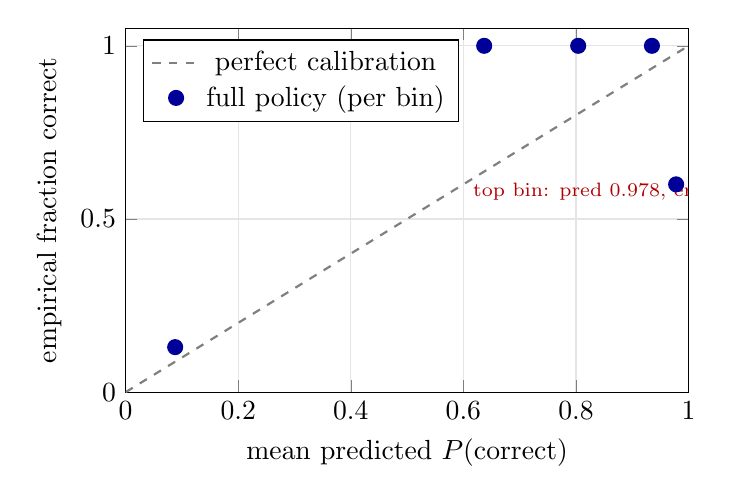
\begin{tikzpicture}
\begin{axis}[
  width=0.72\linewidth, height=6.2cm,
  xlabel={mean predicted $P(\text{correct})$},
  ylabel={empirical fraction correct},
  xmin=0, xmax=1, ymin=0, ymax=1.05,
  legend pos=north west, grid=both, grid style={gray!20},
  every axis plot/.append style={thick},
]
\addplot[domain=0:1, dashed, gray] {x};
\addlegendentry{perfect calibration}
\addplot[mark=*, blue!60!black, only marks, mark size=2.5pt] coordinates {
  (0.088,0.13) (0.637,1.0) (0.804,1.0) (0.935,1.0) (0.978,0.60)
};
\addlegendentry{full policy (per bin)}
\node[anchor=west, font=\scriptsize, red!70!black] at (axis cs:0.60,0.58) {top bin: pred 0.978, emp 0.60};
\end{axis}
\end{tikzpicture}
\caption{Reliability diagram for the \textbf{full} policy. Points on the dashed line
are perfectly calibrated. The top bin sits far \emph{below} the line---severe
over-confidence exactly where a wrong \textsc{accept} costs 20. Caveat: that bin has
only $n=5$ (3/5 correct), so a 95\% Wilson interval spans $\approx0.23$--$0.88$; we
flag the \emph{direction}, not a precise magnitude.}
\label{fig:calib}
\end{figure}

\paragraph{Why this is load-bearing.} The \textsc{accept} threshold in
\S\ref{sec:policy} was derived assuming $\pcorrect$ is the true probability of
\textsf{correct}. If the true rate in the top bin is $0.60$, then the \emph{actual}
expected loss of \textsc{accept} there is $(1-0.60)\times20 = 8$, far above
\textsc{flag}$=2$ and \textsc{reject}$=5$. In that case ``\textsc{accept} at
$\pcorrect\ge0.95$'' would be choosing the \emph{worst} available action: the
miscalibration does not merely add noise, it \emph{inverts} the decision. The
expected-loss policy is only sound once the posterior is calibrated; the $0.95$
threshold is thus a \emph{design target}, not a validated operational risk level.

\subsection{Escalation and the shared blind spot}
Figure~\ref{fig:esc} contrasts average cost with human-review rate. All three policies
commit the \emph{same} two catastrophic wrong-publishes: the two deliberate
\textsf{wrong\_product} seeds, which look normal and even carry cross-source
agreement, are accepted by every policy. The belief layer does not prevent a single
catastrophic error relative to the comparators; its lower average cost comes from
routing 57.5\% of cases to a human (vs.\ 32.5\% baseline, 0\% autonomous).

\begin{figure}[h]
\centering
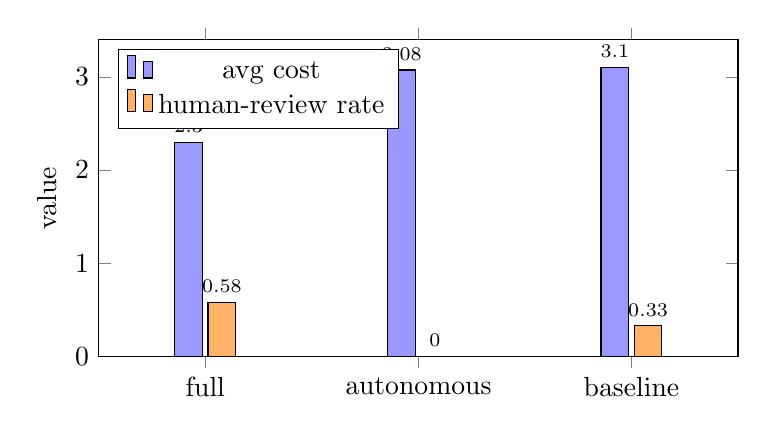
\begin{tikzpicture}
\begin{axis}[
  width=0.8\linewidth, height=5.6cm,
  ybar, bar width=10pt,
  symbolic x coords={full, autonomous, baseline},
  xtick=data,
  ymin=0, ymax=3.4,
  ylabel={value},
  legend pos=north west,
  nodes near coords, nodes near coords style={font=\scriptsize},
  enlarge x limits=0.25,
]
\addplot[fill=blue!40] coordinates {(full,2.30) (autonomous,3.075) (baseline,3.10)};
\addplot[fill=orange!60] coordinates {(full,0.575) (autonomous,0.0) (baseline,0.325)};
\legend{avg cost, human-review rate}
\end{axis}
\end{tikzpicture}
\caption{Average decision cost vs.\ human-review rate. \textbf{full} wins on cost but
at the price of a $57.5\%$ escalation rate; \textbf{autonomous} never escalates yet has
higher \textsc{accept} precision ($0.818$ vs.\ $0.75$). Wrong-publishes are identical
($2/2/2$, not shown), so the cost win is not a catastrophe-reduction win.}
\label{fig:esc}
\end{figure}

\section{Does the belief layer ``earn its keep''?}
\label{sec:earnskeep}

An earlier draft concluded that the belief layer ``earns its keep'' because it beats
the baseline on cost. That conclusion is overstated, and we retract it in favor of a
narrower, defensible one. Three facts, all from our own results, force the correction:

\begin{enumerate}[nosep]
  \item \textbf{Changing decisions $\ne$ better decisions.} Disagreeing with the
        baseline on $37.5\%$ of cases shows the layer \emph{differs}; it does not show
        it is \emph{better}.
  \item \textbf{The win is bought by escalation.} The lower average cost is largely a
        consequence of flagging $57.5\%$ of cases at a flat \textsc{flag} cost of 2. A
        fair comparison must hold the human-review budget fixed---which we have not yet
        done. Indeed the \textbf{autonomous} policy, which never escalates, has
        \emph{higher} \textsc{accept} precision ($0.818$ vs.\ $0.75$).
  \item \textbf{No catastrophe reduction.} All three policies eat the same two
        cost-20 wrong-publishes.
\end{enumerate}

\noindent
\textbf{Honest conclusion.} On a preliminary 40-case sample the full policy showed a
lower average decision cost (2.30 vs.\ 3.10; paired Wilcoxon $p\approx0.015$ but median
per-case difference $0$), primarily by routing $57.5\%$ of cases to human review; it
prevents no more catastrophic wrong-publishes than the baseline. What \emph{is}
supported: the belief layer changes decisions, and---unlike the baseline---it can
\textsc{repair} and pick targeted probes, which are qualitatively different capabilities
that a fixed-escalation-budget experiment on a larger dataset would be needed to price.

\section{Failure modes and limitations}
\label{sec:limitations}

\paragraph{Failure modes (ranked).}
\begin{enumerate}[nosep]
  \item \textbf{\textsf{wrong\_product} blind spot (highest severity).} A value that is
        in-support \emph{and} agrees with sources but is the wrong variant is accepted
        (cost 20). Value $+$ support $+$ agreement cannot catch this; only a
        manufacturer proxy or a human can. Demonstrated by the two failure seeds.
  \item \textbf{Coordinated cross-source error.} The agreement signal assumes source
        independence, which shared upstream feeds violate; five copies of one bad feed
        read as strong (false) agreement.
  \item \textbf{Schema/key mismatch.} If the upstream step mislabels which field a value
        belongs to, the agent cannot recover it (out of scope by assumption).
  \item \textbf{Mislabeled source reliability.} A ``manufacturer'' source that is
        actually a reseller corrupts the prior.
  \item \textbf{Stale support ranges.} New hardware outside the current support range is
        wrongly flagged/rejected (cold-start).
\end{enumerate}

\paragraph{Honest ``what it cannot do.''}
(i) It cannot verify images (pure human-only evidence).
(ii) Its priors are assumed, not counted---there is no general way to prove a strong
prior is justified.
(iii) It cannot detect coordinated cross-source errors.
(iv) Support ranges need ongoing maintenance.
(v) It assumes correct upstream field identification.
(vi) The evaluation is active-learning-biased (\S\ref{sec:threats}).
(vii) \textsc{flag} is modelled as a flat cost 2 that \emph{perfectly} resolves the
case; a real reviewer has an error rate, latency, and a per-item cost that grows with
volume, so the true cost of the full policy's heavy escalation is understated.
(viii) The Bayesian outputs are \emph{conditional on} the assumed priors/likelihoods/costs
and would move if those were re-estimated from labelled data.

\paragraph{Roadmap.} The path to production, out of scope for Week 1: an identity/variant
resolution subsystem (the real fix for the \textsf{wrong\_product} blind spot); an
evidence-lineage/provenance graph or an effective-sample-size discount
$k/(1+(k-1)\rho)$ to replace the hand-tuned agreement discount; loss-aware VOI;
temporal/version/region semantics; an independently-audited gold set including
auto-accepts; risk-tiering of fields and per-product (not per-field) human review; and
recalibration (Platt/temperature/isotonic) before any threshold is used operationally.

\section{Threats to validity}
\label{sec:threats}

\begin{itemize}[nosep]
  \item \textbf{Small sample.} $N=40$ with no confidence intervals; the cost gap is
        significant by a paired test but narrow (median difference $0$). Conclusions are
        preliminary.
  \item \textbf{Active-learning evaluation bias.} The agent auto-accepts a bucket it
        never verifies and only humans see the flagged bucket, so scoring across the
        labelled set over-weights the hard cases and the calibration numbers themselves
        are measured on a biased sample. The honest fix is to randomly audit a slice of
        the auto-accepted bucket and importance-weight it back.
  \item \textbf{Synthetic data.} Cases are generated from the same likelihood model the
        agent uses, which flatters the agent; only the 14 hand-authored cases and the
        deliberate failure seeds inject independent structure.
  \item \textbf{Assumptions drive the numbers.} Because priors/likelihoods/costs are
        assumed, the derived thresholds are internally consistent but not empirically
        validated.
  \item \textbf{Calibration magnitude.} The ``60\% in the top bin'' is $3/5$; the
        direction (over-confidence) is clear, the magnitude is not established at $n=5$.
\end{itemize}

\section{AI-use statement, human discussions, and conclusion}
\label{sec:human}

\paragraph{AI-use statement.} This deliverable was built collaboratively with an AI
coding assistant (Claude, via the Cursor harness) used as a Socratic pair: it taught
the underlying concepts, asked clarifying questions, and drafted files, while the author
owned every design decision (the six worlds, the prior token splits, the cost ordering,
the thresholds, and the buy-stop rule). All conversations, decisions, and their
justifications are logged in \texttt{WORKING-CONTEXT.md}. Three \emph{adversarial} AI
reviews were run in separate sessions across different models---a practitioner review
(ChatGPT), a probability/statistics review (Claude), and a preprint/writing review
(Gemini)---and each comment was adjudicated (accept/reject with a reason) in
\texttt{review-record.md}. The probability review validated the core Bayesian mechanics
and surfaced the conditional-independence and VOI-vs-budget issues; the preprint and
practitioner reviews forced the calibration and ``earns its keep'' honesty corrections
made throughout this paper; the paired significance test was added in direct response
to a reviewer's challenge.

\paragraph{Human discussions.} The design was also shaped by five real online
discussions (documented in \texttt{discussion-record.md}). A web-scraping practitioner's
point---that agreement among sources copying the same feed is not independence---became
the correlated-evidence discount and the \textsf{wrong\_product}/F2 failure analysis; a
machine-learning practitioner's ``build the dumb score-plus-threshold baseline and check
if the belief layer pays rent'' became the \textbf{baseline} decider and the agreement
test; and a statistician's caution about justifying strong priors became the
weakly-informative framing and the label-free prior-predictive calibration idea.

\paragraph{Conclusion.} We presented an explicit, auditable belief-engine decision model
for normalizing scraped product specifications, and we evaluated it honestly. The
framework is sound and the empirical cost advantage is statistically real, but it is
narrow, it is bought by escalation rather than by catching the expensive errors, and it
rests on a posterior that is not yet calibrated in the one bin that matters. The
contribution is therefore a disciplined \emph{way of thinking}---priors with provenance,
asymmetric costs, minimum expected loss, a principled abstain, and a refusal to dress
assumptions up as measurements---rather than a production-ready system. The information
layer (\S\ref{sec:info}) sharpens rather than softens this honesty: it shows that
choosing evidence by expected bits-per-cost reorders our clues, that a highly
informative clue can still be the wrong \emph{buy} (or even raise uncertainty on some
outcomes), and that under our own cost matrix the value of information is usually zero
because guaranteed human review is cheap---so the buy policy was quietly resting on an
optimistic flat human cost. The most valuable next step is not more machinery but
better evidence: a calibrated posterior on an independently-audited sample, a
fixed-escalation-budget comparison at larger scale, and a cost model for the human that
does not treat review as free and infallible.

\appendix
\section{Required core questions}
\label{app:core}
Answers in the author's own words, grounded in this problem wherever possible.

\begin{enumerate}[itemsep=3pt]
\item \textbf{Hidden state, and ours?} A fact the agent cannot observe at decision
time but needs in order to act. Ours is \emph{which of six worlds} produced a scraped
value---\textsf{correct}, \textsf{unit\_error}, \textsf{wrong\_product}, \textsf{typo},
\textsf{missing}, \textsf{garbled}---since the true canonical spec is never seen.

\item \textbf{Why is directly predicting an answer insufficient?} A point prediction
(``it's a typo'') throws away how \emph{sure} we are and which alternatives are live,
which is exactly what an asymmetric cost matrix needs. Predicting ``correct'' with 55\%
confidence and with 95\% confidence should lead to different actions; a bare label
cannot express that.

\item \textbf{Belief distribution, and why sum to one?} A probability over all hidden
worlds representing our current uncertainty. It sums to one because the worlds are
exhaustive (\S\ref{sec:worlds})---the true value is \emph{some} world, so the total
probability of ``it is one of them'' must be $1$.

\item \textbf{Prior vs.\ posterior?} The prior is the belief before this field's clues
(our source-reliability board, e.g.\ $\pcorrect=0.50$ on a mid source); the posterior
is the belief after applying a clue via Bayes (e.g.\ $\pcorrect=0.089$ after the
out-of-support signal).

\item \textbf{Likelihood vs.\ probability?} Likelihood is $P(\text{clue}\mid
\text{world})$---how naturally each world would \emph{produce} the observed clue---read
as a function of the world for fixed evidence, so it need not sum to one across worlds.
A probability (e.g.\ the posterior) is normalized over worlds.

\item \textbf{What does agent uncertainty mean?} That its belief mass is spread over
several worlds rather than concentrated on one; operationally, that no single terminal
action is clearly cheapest. Our post-oos belief is uncertain: three error worlds remain
live.

\item \textbf{Entropy, and why it is uncertainty?} $H=-\sum_w b(w)\log_2 b(w)$: the
average number of yes/no questions needed to pin down the world. It is maximal when
belief is uniform (maximum confusion) and zero when one world has all the mass
(certainty), so it \emph{is} a measure of doubt.

\item \textbf{A bit, plainly?} One yes/no question's worth of uncertainty---the doubt in
a fair coin flip. Eight equally likely options are three bits because three good
halving questions identify the answer.

\item \textbf{Information gain vs.\ entropy?} Information gain is the drop in entropy
from receiving evidence. \emph{Expected} gain $=H(\text{prior})-H(W\mid\text{clue})$;
on our case the out-of-support clue's expected gain is $0.228$ bits.

\item \textbf{Conditional entropy?} $H(W\mid\text{clue})$: the entropy we \emph{expect}
to remain after a clue, averaged over its possible outcomes weighted by their
probabilities ($0.112\cdot1.880+0.888\cdot1.897=1.895$ bits here). Information gain is
the starting entropy minus this.

\item \textbf{Mutual information vs.\ correlation?} Mutual information is the expected
information one variable gives about another (identical to expected information gain);
it is zero only under independence and captures \emph{any} dependence. Correlation only
captures \emph{linear} co-movement, so a variable and its square can have zero
correlation yet full mutual information.

\item \textbf{KL divergence, and why not a distance?} $\mathrm{KL}(p\|q)=\sum p\log_2
\tfrac{p}{q}$ measures the extra bits paid for coding samples from $p$ using a code
built for $q$. It is not a distance because it is asymmetric and violates the triangle
inequality; it is zero iff $p=q$.

\item \textbf{Why KL asymmetric? Small example?} Because it weights the gap by $p$, the
``true'' side. With $p=(0.9,0.1)$ and $q=(0.5,0.5)$, $\mathrm{KL}(p\|q)\approx0.53$
bits, but $\mathrm{KL}(q\|p)\approx0.74$ bits---swapping the arguments changes the
penalty, since regions where $p$ is large but $q$ is small hurt most.

\item \textbf{Jensen--Shannon, and why introduced?} $\mathrm{JS}(p,q)=\tfrac12
\mathrm{KL}(p\|m)+\tfrac12\mathrm{KL}(q\|m)$ with $m=\tfrac12(p+q)$. It was introduced
to fix KL's flaws: it is symmetric, always finite (no divide-by-zero when one
distribution has zero mass), and its square root is a true metric---useful for
comparing, e.g., two sources' value distributions for the same field.

\item \textbf{Calibration, and why it matters?} An agent is calibrated if things it
calls 90\%-likely happen about 90\% of the time. It matters because our expected-loss
math trusts the numbers: our top confidence bin is only $\sim$60\% correct, which (if
real) inverts the \textsc{accept} decision the threshold was meant to license
(\S\ref{sec:results}).

\item \textbf{Expected cost, and how we derived the threshold?} Expected cost of an
action $=\sum_w b(w)\,C(\text{action},w)$. Since \textsc{accept} costs $20$ if wrong and
\textsc{flag} a flat $2$, \textsc{accept} wins only when $(1-\pcorrect)\cdot20<2$, i.e.\
$\pcorrect>0.90$---so $90\%$ is the cost-\emph{derived} floor (we operate at $95\%$ for
margin).

\item \textbf{Value of information; when is more not worth it?} VOI is the expected
reduction in decision loss from a clue, and you buy only if VOI exceeds the clue's cost.
It is not worth it when no outcome would change the chosen action---on our worked case
\textsc{flag} at $2$ dominates in every branch, so VOI$=0$ and the agent should flag,
not buy (\S\ref{sec:info}).

\item \textbf{Can a question be informative yet useless? Our example.} Yes. The
manufacturer proxy is our \emph{most} informative clue ($0.250$ bits) yet has VOI$=0$
on the $160$\,GB case, because whatever it returns, \textsc{flag} stays
cheapest---informative, but it changes no action, so it is useless \emph{there}.

\item \textbf{Distribution shift, and detection?} When the world the model was tuned on
stops matching reality (a new category, a new copying pattern). Our agent could detect
it by prior-predictive monitoring---if the observed rate of out-of-support values,
empties, or cross-source disagreement drifts from what the priors/likelihoods predict
(the $P(\text{clue})$ normalizer), the assumptions are stale.

\item \textbf{When to stop and act? The rule.} Act when any fires: (i) one terminal
action's expected loss is clearly lowest (belief is decisive); (ii) no affordable clue
is VOI-positive; (iii) two buys stop moving the posterior (correlated evidence);
otherwise buy the highest positive-$(\text{VOI}-\text{cost})$ clue and re-evaluate
(\S\ref{sec:info}).
\end{enumerate}

\bibliographystyle{plain}
\bibliography{references}

\end{document}
